\chapter{Experimental Strategy }


\textit{%To investigate the problem statement multiple experiments were developed using a lab-scale NF filtration system, developed in collaboration with Grundfos.
A lab-scale NF filtration system was provided by Grundfos and will be used to investigate the rejection of NF of chloride and silica. 
The lab-scale NF system will be described in the following chapter, and experiments discussed in this chapter will be performed using this lab-scale set up. 
Results and observations based on experiments presented in this chapter will be basis for development of \textcolor{blue}{"The model"} to describe rejection of chloride and silica in NF.
}


\section{Lab-Scale Filtration Setup}

Experiments performed in relation to this project will be  filtration on a lab-scale setup developed in collaboration with Grundfos. 
A lab-scale set up is a scaled down version which allow for a smaller water volume and easier control of parameters. 
%and experiments were conducted in order to understand the processes which could later be scaled to a pilot plan filtration system. 
All filtration were performed using a lab-scale hollow fiber, inside-out NF membrane obtained by NXFiltration (MexFil MPO25 dNF40). 
%optimal operation condition for the the lab-scale dNF40 membrane is listed in \rod{appendix: membrane_stads}.
%This membrane was selected based on internal work at Grundfos, 
This membrane achieve high rejection of divalent ions at 91\% for \ce{MgSO4}, and is robust with a wide range for operational conditions, see \textcolor{blue}{appendix: membrane stads}. 
The lab-scale NF membrane was operated in cross-flow mode due to the membrane configuration, to achieve high permeate flux, and reduce fouling. 
The hollow fiber configuration leads to a large active membrane area in a compact membrane configuration. \textcolor{blue}{kilde på det}
The active surface area is \SI{0.05}{\square\meter} with a cylindrical module size of 30 cm long and a 2.4 cm diameter. 
There is some uncertainty related to the size of the active membrane surface area, as it is difficult to precisely determine by the manufacturer.  \citep{Datasheet_dNF40_labscale_2019}


%The filtration system is operated in cross-flow mode due to the membrane configuration of hollow fiber, and to reduce fouling.
%ekstra noter: 
%sufficient at removing divalent ions and dissolved organics such as micro pollutants.
%as it is one of the only NF hollow fiber membranes commercially avaliable on the market.
% \begin{table}[H]
% \centering
% \caption{Membrane specifications from dNF40 lab-scale membrane \citep{Datasheet_dNF40_labscale_2019}}
% 	\begin{tabular}{c|c}
%     Membrane material & Modified PES \rod{MODIFIED WITH WHAT}  \\ 
%     Molecular Weight Cut Of (MWCO) & 400 Da  \\
%     Membrane charge at pH 7 &  Negative \\
%      Max system pressure  & 6 bar  \\
%      Max temperature (operation) & 40 \degree C \\
%     pH range (operation)  & 2-12  \\
%      pH range (cleaning) &  1-13 \\
%      Cross-flow velocity range  & 0.1-2.0 $m/s$  \\
%      Membrane surface area & 0.05 $m^2$\\
%      Permeability  & ? \\
% 	\end{tabular}
% 	\label{Tab:stats_membran}
% \end{table}

%See \Cref{fig:PID_system} for a overview of the filtration setup.
%\rod{ryk rundt så det der er fysisk til stede kommer først, og operation kommer til sidst. }


The lab-scale filtration system was designed, 
%were both single pass and batch experiments were possible. 
so the system could be operated semi-automated, by the use of a PLC programmed to operate valves and pumps along with collecting data every second from various sensors, see \textcolor{blue}{figure for illustrtion of lab-scale set-up}.
Two Grundfos dosing pumps (SMART Digital XL 60 L/h) were used to generate feed flow, as well as a dosing pump for the peameate side for backwash.
The system had a \SI{100}{\micro\meter} pre-filter installed to remove larger particulates before the NF membrane.
A magnetic flow meter measured the feed flow rate and was used to regulate the crossflow velocity.
Due to the usage of dosing pumps, pulsation dampeners were present to the system to reduce pulsation in the flow.
In order to monitor and control the filtration process and performance multiple sensors were present in the system. 
Pressure sensors were placed on the feed, retentate and permeate sides of the membrane to monitor the TMP. 
%Information from these sensors was used to estimate current membrane performance and to monitor degrading membrane performance to know when mechanical or chemical cleaning was necessary.
Conductivity sensors were present before and after the membrane.
This allowed using the conductivity measurements as a first approach to determine ion rejections and membrane performance. 
pH sensors were placed on the feed side of the membrane to monitor changes in pH of the feed solution. 
%The filtration system including various gauges and valves is illustrated on \Cref{fig:PID_system}.
A custom regulation-valve controlled the flow of the retentate stream by constricting the tubing via a motorized actuator, this allowed for pressure regulation. 
%The pressure regulation was achieved by this valve as the feed flow was more or less constant and the retentate tube became constricted.
%The system was operated in constant flux mode, where the system regulated the pressure to maintain a constant water flux over the membrane.
The permeate flow rate was determined by continuously weighing the accumulated permeate on a scale \textcolor{blue}{[stads på vægt]} and averaging over a time period.  
Based on this lab scale experimental setup operation in either batch process or single-pass is possible.

Internal work at Grundfos has investigated ideal filtration parameters, which have been used to run a larger pilot scale NF filtration set-up, which will be elaborated in \rod{ref til chapter omkring NF pilot}. %present at Grundfos. 
%Results from previous work done at Grundfos, found that a flux above 20 LMH and cross flow above 0.5 m/s does not yield significantly higher rejection based on conductivity \citep{Sebastians_master_2020}.
The filtration parameters selected and scaled for the lab-scale experimental set-up will therefore be determined to best resemble that of the pilot scale NF filtration set up.
These filtration parameters are always constant with permeate flux at 20 LMH and crossflow velocity 0.5 m/s. 
When operating in batch mode water recovery should be above 90 \%. 



%Permeate flux was 20 LMH at cross flow velocity of 0.5 m/s, these parameters match the pilot scale system.
%Always constant: Flux (permeate flow),Feed flow (Crossflow),
%The filtration parameters were selected to best resemble a pilot scale NF plant present at Grundfos.
%, where only some of these parameters are possible to mimic for a lab scale system. 

\begin{figure}[h]
    \centering
    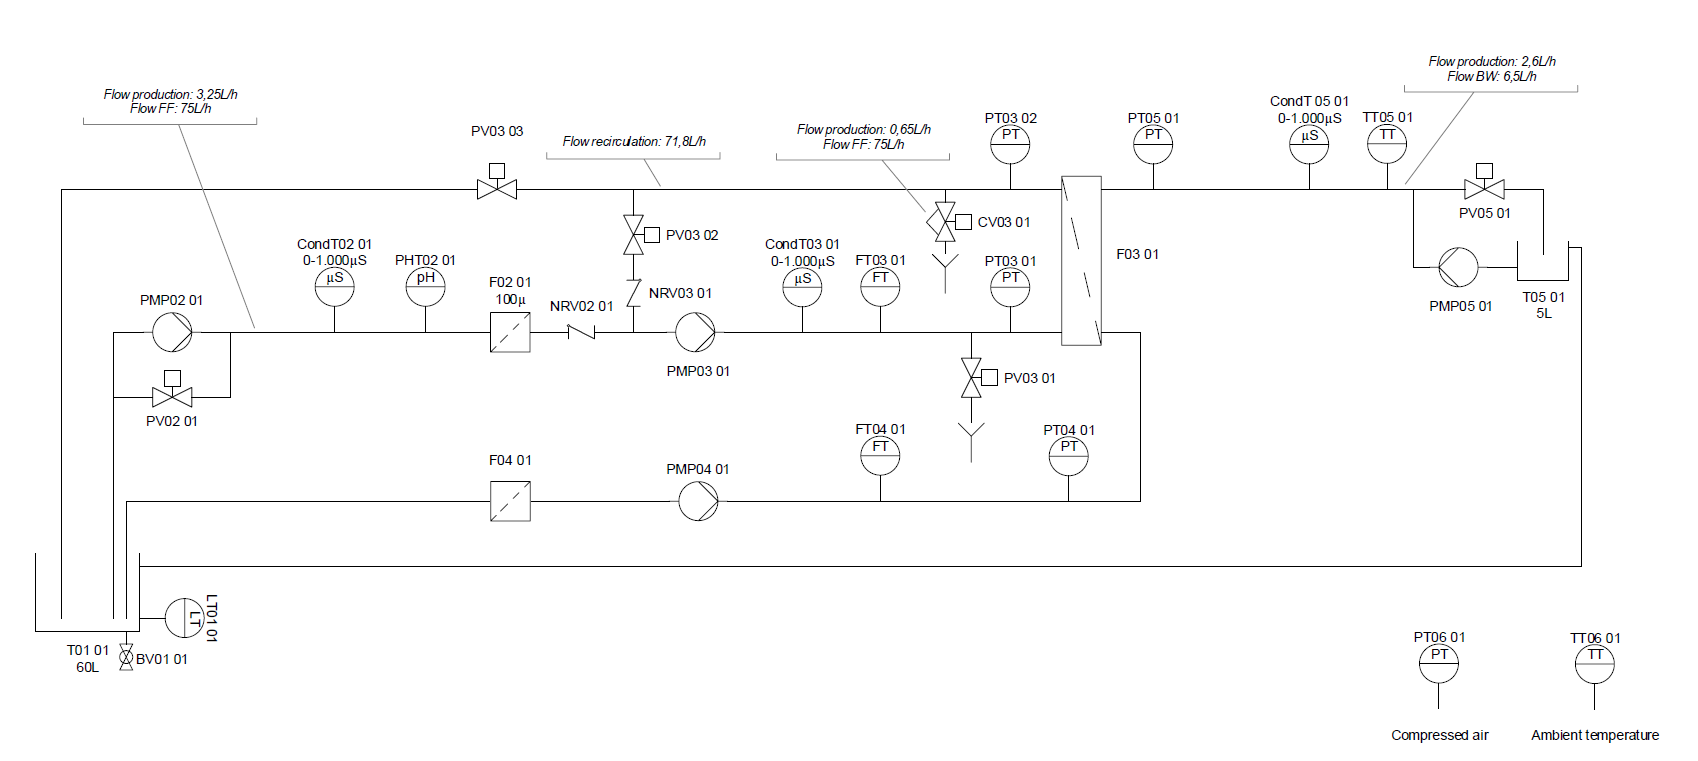
\includegraphics[width=0.9\textwidth]{Billeder/exp/PID.png}
    \caption{Pi \& D Diagram of 'the system'}
    \label{fig:PID_system}
\end{figure}






% \begin{ceqn}
% \begin{align}
%     Rec = Q_p/Q_f = 17[L/h]/1173[L/h] = 0.014 = 1.4 \%
% \end{align}
% \end{ceqn}

% \textcolor{blue}{Se steffens udregniner om sammenlingning af NF mega og NF mini parametre, noget vi skal se mere på? }

% \begin{figure}
%     \centering
%     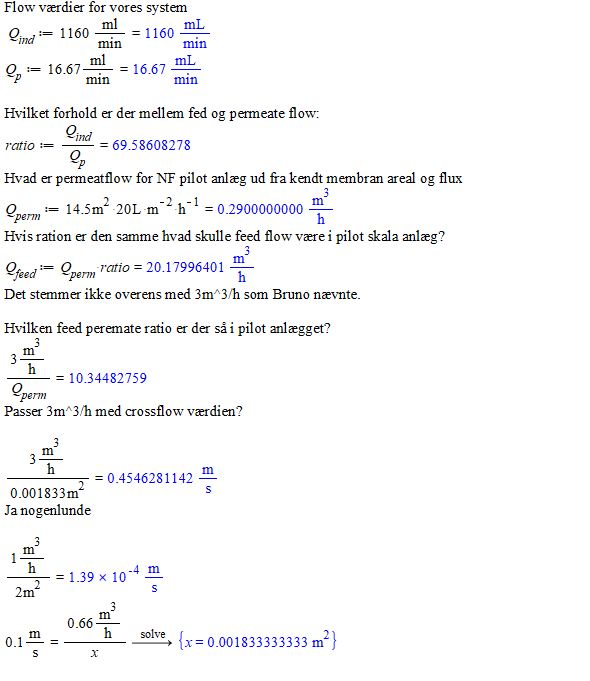
\includegraphics[width=0.7\textwidth]{Billeder/exp/godt_og_blandet_fra_maple.png}
%     \caption{Lidt udregninger omkring NF mini vs NF Mega}
%     \label{NF_mini_vs_mega}
% \end{figure}



\subsection{Membrane Cleaning}
% \begin{itemize}
%     \item hydraulic cleaning once pr. hour. 
%     \item irreversible fouling on membrane can be removed by cleaning in place (CIP) 
%     \item backwash use permeate water. 
% \end{itemize}

Cleaning of the membrane is necessary over time to remove fouling, and can be divided into two categories; Hydraulic cleaning and chemical cleaning. \citep{NXfiltration_operation_manual} 
For experiments performed on the lab-scale filtration system, hydraulic cleaning will be performed between filtration with 5 min flush at 1000 ml/min. 
This helps remove solids which are present on the membrane surface \citep{NXfiltration_operation_manual}.  
Following a 15 min backwash with \textcolor{blue}{600 ml/min ??} is performed where permeate quality water flows through the membrane in opposite direction this helps remove foulants. \citep{NXfiltration_operation_manual}
%Feed or tap water will be used for flush during hydraulic cleaning. 


%The preferred regular hydraulic cleaning is flush, where solids which lie on the membrane surface can be removed by flushing the membrane with water at higher velocity than used during filtration. 
%The flush should take place for minimum 1-2 minutes and the permeate water is the preferred water quality but feed water can also be used. 
%As a supplement to flush backwash can be used as a hydraulic cleaning to maintain an acceptable permeability.
%In backwash water of permeate quality  flow through the membrane in opposite direction of filtration, and remove foulants from the membrane surface.  
%It is recommended to perform backwash with similar flux rate as filtration flux. \textcolor{blue}{KILDE = lang manual fra NXfiltration}


If hydraulic cleaning is not sufficient to remove foulants, a chemical cleaning can be performed. 
%A chemical cleaning should be performed if the TMP increase to higher than 30 \% of start-up values.  
A chemical cleaning can be performed in the form of chemically enhanced flush (CEF), where chemicals are dosed to the feed side of the membrane during a flush.  \citep{NXfiltration_operation_manual} 
%When performing a CEF an alkaline cycle using sodium hydroxide to reach pH 11.5-12 in combination with sodium hypochlorite for disinfection has proven effective in removing organic fouling. Where a cycle using an acid flush is effective at removing precipatation of salt.    textcolor{blue}{KILDE = lang manual fra NXfiltration}
Chemical cleaning will be performed between different experiments to ensure best membrane performance, or if scaling or high increase in TMP is observed. 
The chemical cleaning is designed based on NXfiltrations recommendation \citep{NXfiltration_operation_manual} as well as internal practice within Grundfos. 
Due to the size of the lab-scale a volume of 3 liter of each cycle is prepared. 
An alkaline cycle is prepared with 20 mM Sodium Hydroxide to increase pH to 11.5-12 and 2.7 mM Sodium Hypochlorite.  
This alkaline cycles is intended to disinfect and  remove organic fouling, where as an acidic cycle remove precipitated salts  \citep{NXfiltration_operation_manual}. 
An acidic cycle is prepared with %0.1 mM eller 1 mM 
Citric acid to pH 2 and heated to 40 \textdegree{}C. 
Each cycle is flushed for a minimum of 15 min, longer if needed. 
Before and after each cycle the system is flushed with RO-water to ensure that no chemicals are left in the system. 








